\documentclass{beamer}
\usetheme{Luebeck}
\usecolortheme{seahorse}
\usefonttheme{structurebold,serif}
\setbeamertemplate{navigation symbols}{\usebeamerfont{footline}\insertframenumber/\inserttotalframenumber}
\usepackage{luatexja-fontspec}
\setmainfont{DejaVu Serif}[Scale=0.9]
\setsansfont{DejaVu Sans}[Scale=0.9]
\setmonofont{DejaVu Sans Mono}[Scale=0.9]
\setmainjfont{YuKyo_Yoko-Medium}[BoldFont=YuKyo_Yoko-Bold]
\setsansjfont{YuGo-Medium}[BoldFont=YuGo-Bold]
\usepackage{hyperref}
\usepackage[bold-style=ISO]{unicode-math}
\usepackage{graphicx}

\newcommand{\ii}{\mathrm{i}}
\newcommand{\jj}{\mathrm{j}}
\newcommand{\kk}{\mathrm{k}}

\title{四元数と回転}
\author{宇佐見 公輔}
\date{2022年1月22日}
\begin{document}
\maketitle

\begin{frame}
    \frametitle{自己紹介}
    宇佐見 公輔(うさみ こうすけ)
    \begin{itemize}
        \item 職業:プログラマ
        \item 趣味:数学
    \end{itemize}

    \bigskip
    今日の話に関連する過去の登壇:
    \begin{itemize}
        \item 四元数のはなし(2020年5月 / 関西日曜数学友の会)
        \item 八元数のはなし(2021年10月 / 日曜数学会)
    \end{itemize}
\end{frame}

\begin{frame}
    \frametitle{自己紹介}
    近況:\\
    \begin{itemize}
        \item 今年から、株式会社ゆめみ所属
    \end{itemize}

    \bigskip
    ゆめみメンバーによるグループLiberal Arts Labの紹介:
    \begin{itemize}
        \item 2月3日:タカタ先生のお笑い数学全史・第十四章\\produced by Liberal Arts Lab ×日本お笑い数学協会
        \item 2月24日:「僕の本、こう活かそう!」〜数学のお兄さんの書籍を使った算数・数学の学び方〜\\produced by Liberal Arts Lab ×日本お笑い数学協会
    \end{itemize}
\end{frame}

\begin{frame}
    \frametitle{四元数とは}
    \begin{block}{四元数}
        \(x_0+x_1\ii+x_2\jj+x_3\kk\)(\(x_i\in\mathbb{R}\))とあらわされる数。
        \begin{gather*}
            \ii^2=\jj^2=\kk^2=-1\\
            \ii\jj=-\jj\ii=\kk,\quad\jj\kk=-\kk\jj=\ii,\quad\kk\ii=-\ii\kk=\jj
        \end{gather*}
    \end{block}
    \begin{itemize}
        \item 加減乗除が可能(特に除法が可能)。
        \item 分配法則、結合法則、加法の交換法則が成り立つ。
        \item 乗法の交換法則が成り立たない。
    \end{itemize}
\end{frame}

\begin{frame}
    \frametitle{四元数の大きさ}
    \begin{block}{四元数の大きさ(絶対値)}
        \(x=x_0+x_1\ii+x_2\jj+x_3\kk\)(\(x_i\in\mathbb{R}\))の大きさ\(|x|\)は、
        \[
            |x|=\sqrt{x_0^2+x_1^2+x_2^2+x_3^2}
        \]
        で、大きさは乗法によって保たれる。
        \[
            |xy|=|x||y|
        \]
    \end{block}
    \begin{itemize}
        \item ハミルトンは、この性質が成り立つようなものを探した結果、三元数を作ることはできず、四元数になった。
    \end{itemize}
\end{frame}

\begin{frame}
    \frametitle{2次元平面上の回転}
    \begin{block}{2次元平面上の回転}
        複素数\(x=x_0+x_1\ii\)に大きさ\(1\)の複素数\(q\)をかける操作は、2次元平面上の回転をあらわす。
        \[
            x\mapsto qx
        \]
    \end{block}
    \begin{itemize}
        \item \(|qx|=|q||x|=|x|\)なので原点からの距離が保たれる。
    \end{itemize}
    \begin{center}
        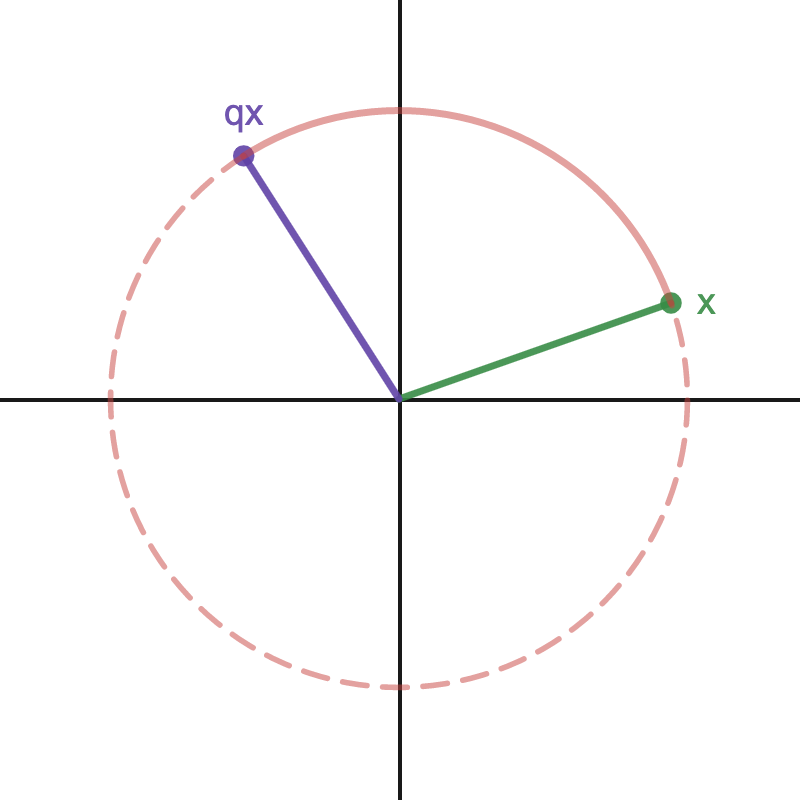
\includegraphics[scale=0.12]{RotateComplex.png}
    \end{center}
\end{frame}

\begin{frame}
    \frametitle{4次元空間上の回転}
    \begin{block}{4次元空間上の回転}
        四元数\(x=x_0+x_1\ii+x_2\jj+x_3\kk\)に大きさ\(1\)の四元数\(q\)をかける操作は、4次元空間上の回転をあらわす。
        \[
            x\mapsto qx
        \]
    \end{block}
    \begin{itemize}
        \item \(|qx|=|q||x|=|x|\)なので原点からの距離が保たれる。
    \end{itemize}
    \begin{center}
        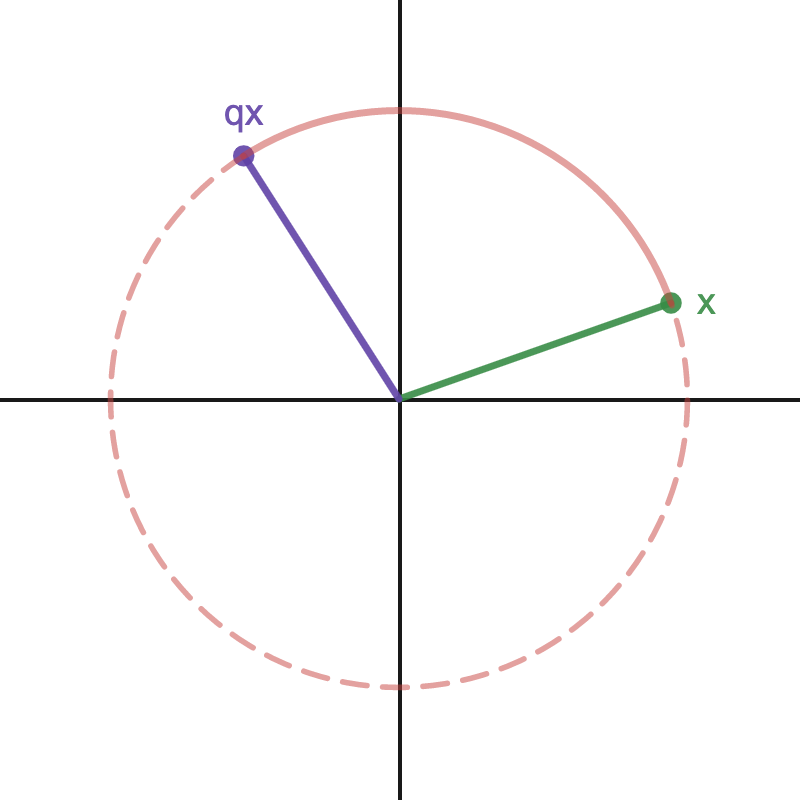
\includegraphics[scale=0.12]{RotateComplex.png}
    \end{center}
\end{frame}

\begin{frame}
    \frametitle{3次元空間を考える}
    ハミルトンは3次元空間上の回転を表現する方法が欲しかったのだが、三元数は作れなかった。

    \bigskip
    四元数は4次元空間の点に対応する。
    \[
        x_0+x_1\ii+x_2\jj+x_3\kk\leftrightarrow(x_0,x_1,x_2,x_3)
    \]
    四元数の虚数部だけを使うことにして(純虚四元数)、3次元空間と対応するようにしてみる。
    \[
        x_1\ii+x_2\jj+x_3\kk\leftrightarrow(x_1,x_2,x_3)
    \]
\end{frame}

\begin{frame}
    \frametitle{純虚四元数}
    純虚四元数は残念ながら乗法で閉じていない。
    \begin{align*}
        &(x_1\ii+x_2\jj+x_3\kk)(y_1\ii+y_2\jj+y_3\kk)\\
        =&-(x_1y_1+x_2y_2+x_3y_3)\\
        &+(x_2y_3-x_3y_2)\ii+(x_3y_1-x_1y_3)\jj+(x_1y_2-x_2y_1)\kk
    \end{align*}
    そのため、単純に乗法で3次元空間上の回転を表現することはできない。
\end{frame}

\begin{frame}
    \frametitle{3次元空間上の回転}
    実は次のように表現することができる。
    \begin{block}{3次元空間上の回転}
        純虚四元数\(x=x_1\ii+x_2\jj+x_3\kk\)に対して、大きさ\(1\)の四元数\(q\)を使った次の操作は、3次元空間上の回転をあらわす。
        \[
            x\mapsto qxq^{-1}
        \]
    \end{block}
    \begin{itemize}
        \item \(qxq^{-1}\)は純虚四元数になる。
    \end{itemize}
\end{frame}

\begin{frame}
    \frametitle{3次元空間上の回転とは}
    3次元空間上での回転を少し噛み砕いて考えてみる。

    \bigskip
    2次元平面上の原点中心の回転は、角度だけで決まっていた。\\
    3次元空間上の原点中心の回転は、それに加えて「どの方向に回転させるか」の情報がないと決まらない。
    言い方を変えると、「どの平面上で回転させるか」とも言える。
    
    \bigskip
    つまり、3次元空間上の原点中心の回転は、平面を指定する法線ベクトル\(n\)と、
    その平面上で回転させる角度\(\theta\)との2つの情報で決まる。

    \bigskip
    (こういうことをビジュアライズする能力が欲しい・・・)
\end{frame}

\begin{frame}
    \frametitle{3次元空間上の回転(再)}
    \begin{block}{3次元空間上の回転}
        点\(X=(x_1,x_2,x_3)\)を法線ベクトル\(n=(n_1,n_2,n_3)\)(ただし\(|n|=1\)とする)で決まる平面上を\(\theta\)だけ回転させる操作を考える。

        \bigskip
        純虚四元数\(x=x_1\ii+x_2\jj+x_3\kk\)に対して、大きさ\(1\)の四元数
        \[
            q=\cos\frac{\theta}{2}+\left(\sin\frac{\theta}{2}\right)(n_1\ii+n_2\jj+n_3\kk)
        \]
        を使った次の操作
        \[
            x\mapsto qxq^{-1}
        \]
        は、上述の3次元空間上の回転をあらわす。
    \end{block}
\end{frame}

\begin{frame}
    \frametitle{3次元空間上の回転の不思議}
    実際に回転であることの説明はここではしないけれど、
    3次元空間の点と純虚四元数との対応を念頭に置いて、
    変換\(x\mapsto qxq^{-1}\)が回転になっているらしいというのを飲み込んだとして。

    \bigskip
    さらに考えてみると、大きさ\(1\)の四元数を集めた集合は、乗法で群をなす。
    \(x\mapsto qxq^{-1}\)という操作は、群の言葉でいえば共役をとる操作。
    純虚四元数に対して、大きさ\(1\)の四元数の群の元で共役をとるのが、回転変換あるいは鏡映変換に対応すると考えられる。

    \bigskip
    それでも、\(x\mapsto qxq^{-1}\)という操作は、ちょっと不思議な感じがする。
\end{frame}

\begin{frame}
    \frametitle{3次元空間上の回転の不思議}
    \(x\)と\(qxq^{-1}\)は純虚四元数であり、3次元空間の点と対応している。
    しかしその過程で出てくる\(qx\)あるいは\(xq^{-1}\)は純虚四元数ではない。

    つまり、3次元空間上の回転をあらわすために、一度4次元の世界に飛び出している。

    \bigskip
    左から\(q\)をかける操作で、実軸方向に\((q|x)\)だけずれた世界で、外積\(q\times x\)をとる。

    そこに右から\(q^{-1}\)をかける操作で、実軸方向にずらして元の世界に戻ってきて、外積をとる。

    これが実は回転になっているというのである。不思議な感じがしませんか?
\end{frame}

\begin{frame}
    \frametitle{参考文献}
    結論的な話がない感じですが、参考文献を挙げておきます。

    \bigskip
    これらには先ほどの操作が3次元空間をあらわすことの証明や説明が書かれています。
    \begin{itemize}
        \item 松岡 学「数の世界 自然数から実数、複素数、そして四元数へ」講談社ブルーバックス
        \item 矢野 忠「四元数の発見」海鳴社
        \item 今野 紀雄「四元数」森北出版
    \end{itemize}
\end{frame}

\end{document}
